\setchapterimage[2cm]{../images/header-stx.jpg}
%\setchapterpreamble[u]{\margintoc}
\chapter{Sunflower-saxitoxin complexes}
\labch{stx}

\begin{marginfigure}
    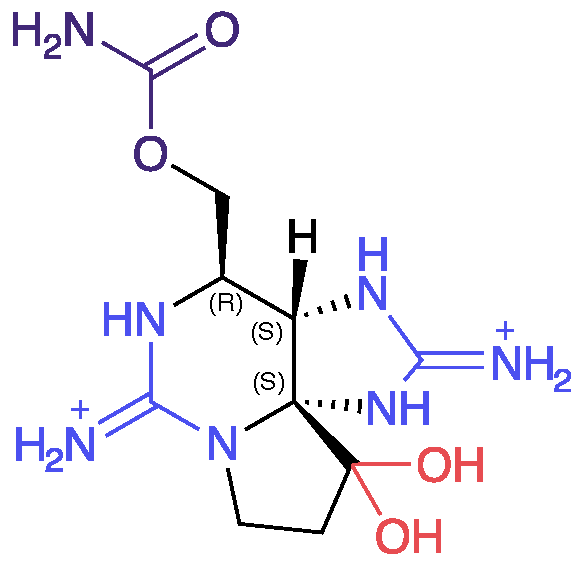
\includegraphics{stx-structure}
    \caption[Structure of STX]{Structure of STX}
    \labfig{stx-structure}
\end{marginfigure}

Having obtained a general characterization of the sunflower-type molecules, it's time to get back to the problem at hand and start looking into how they can be applied.

Let's reintroduce the molecule that motivated this whole study: saxitoxin (STX).
For the purposes of this study, the STX structure features two guanidinium moieties (which are protonated due to the simulation of acidic conditions), two hydroxyl, and one carbamate group as it can be seen in \reffig{stx-structure}.

\blindtext

\section{Spectroscopic study of lone STX}

\blindtext[3]

\section{Study of adsorption}

After having characterized the spectroscopic profile of STX, it's time to assess its interactions with the members of the sunflower family, keeping in mind that the main goal of this work is determining if any of them could be a SERS substrate suitable for its detection.
The first study that must be carried out, before any spectroscopic technique can be applied, is that of adsorption: how does STX adheres to the flowers, how stable is the resulting complex, what is the nature of that interaction...
This is a crucial matter, as there's no point in calculating spectra for a system that isn't stable.

\subsection{Sampling and optimization}

\begin{margintable}
    \centering
    \caption[Energies of STX-S08 conformers]{Relative energies of the STX-S08 conformers, with respect to the most stable one}
    \begin{tabular}{@{}l
                       S[table-format=2.3]@{}}
        \toprule
        System ID & {Rel. E (\si{\kilo\calorie\per\mole})} \\
        \midrule
        STX-S08-1 & 0.000 \\
        STX-S08-2 & 1.337 \\
        STX-S08-9 & 7.133 \\
        STX-S08-7 & 7.504 \\
        STX-S08-6 & 9.896 \\
        STX-S08-4 & 18.554 \\
        STX-S08-3 & 20.321 \\
        STX-S08-10 & 21.734 \\
        STX-S08-5 & 22.529 \\
        STX-S08-8 & 29.715 \\
    \end{tabular}
    \labtab{stx-s08-energies}
\end{margintable}

In order to take into account the possible conformational variability, the STX was manually given an array of different relative positions and angles with respect to the surface of the flowers.
Following this idea, 10 different variations were modeled for each of the 18 STX-sunflower pairs, resulting in a total of 180 structures.
These various orientations will be referred to as \q{conformers}.
All of the conformers for each pairing were optimized at the M06-2X/def2SVP calculation level, and their final energies were compared in order to identify the most stable ones and discard the unstable.
Taking the STX-S08 system as an example, the relative energies of all of its generated conformers are displayed in \reftab{stx-s08-energies}.
As it can be seen, the most stable conformer (MSC) is STX-S08-1.
However, STX-S08-2, STX-S08-9 and STX-S08-7 are also close energy-wise.
A question arises, how can we determine which conformers are stable enough to be important, and which are not?

\begin{figure}
    \includegraphics{s08-conformers}
    \caption[Conformers of STX-S08]{Examples of conformers of the STX-S08 system, from left to right, STX-S08-1, STX-S08-9, and STX-S08-3}
    \labfig{s08-conformers}
\end{figure}

\begin{margintable}
    \centering
    \caption[Maxwell-Boltzmann populations of STX-S08]{Maxwell-Boltzmann populations of the STX-S08 conformer set, expressed as percentages}
    \begin{tabular}{@{}l
                       S[table-format=2.2]@{}}
        \toprule
        System ID & {Population (\si{\percent})} \\
        \midrule
        STX-S08-1 & 58.56 \\
        STX-S08-2 & 34.16 \\
        STX-S08-9 & 3.30 \\
        STX-S08-7 & 2.83 \\
        STX-S08-6 & 1.08 \\
        STX-S08-4 & 0.03 \\
        STX-S08-3 & 0.02 \\
        STX-S08-10 & 0.01 \\
        STX-S08-5 & 0.01 \\
        STX-S08-8 & 0.00 \\
    \end{tabular}
    \labtab{stx-s08-populations}
\end{margintable}

\subsection{Maxwell-Boltzmann statistics}
Our answer to this problem consisted in applying Maxwell-Boltzmann statistics to transform these energies into population fractions.
This concept essentially translates as the fraction of each conformer that would be present in a macroscopic sample at a certain temperature.
As modeled in \refeq{maxwell-boltzmann}, $p_i$ represents the population fraction of the conformer $i$, while $p_\textit{MSC}$ is the fraction of the MSC of that particular set of conformers.
As for the rest of the elements of the equation, $\varepsilon$ corresponds to the absolute energies of the systems, $N$ is the total number of conformers in each set (which is 10 in our case), $k$ is Boltzmann's constant, and $T$ is the temperature of the system in \si{\kelvin} (which for the purposes of this study is set at \fix{\SI{298}{\kelvin}, or is it 273??}).

\begin{align}
\begin{split}
    \labeq{maxwell-boltzmann}
    \frac{p_i}{p_\textit{MSC}}&=e^{\varepsilon_\textit{MSC}-\varepsilon_i/kT} \\
    \sum_{i=1}^{N}\frac{p_i}{p_\textit{MSC}}&=\frac{\sum_{i=1}^{N}p_i}{p_\textit{MSC}}=\frac{1}{p_\textit{MSC}} \\
    \frac{p_i/p_\textit{MSC}}{1/p_\textit{MSC}}&=\frac{e^{\varepsilon_\textit{MSC}-\varepsilon_i/kT}}{\sum_{i=1}^{N}\frac{p_i}{p_\textit{MSC}}}=p_i \\
\end{split}
\end{align}

Continuing with the example, the populations for STX-S08 were computed and are displayed in \reftab{stx-s08-populations}.
As an arbitrary threshold, it was decided to filter out all of the conformers with populations lower than \SI{1}{\percent}, and to just keep studying the remaining ones.

\begin{table}
    \centering
    \caption[Maxwell-Boltzmann populations for all sets]{Maxwell-Boltzmann populations for all sets, as percentages}
    \begin{tabular}{@{}c
                    S[table-format=2.2]
                    S[table-format=2.2]
                    S[table-format=2.2]
                    S[table-format=2.2]
                    S[table-format=2.2]
                    S[table-format=2.2]@{}}
        \toprule
        System & {S} & {Se} & {As} & {AsN} & {P} & {PN} \\
        n of petals & {\si{\percent}} & {\si{\percent}} & {\si{\percent}} & {\si{\percent}} & {\si{\percent}} & {\si{\percent}} \\
        \midrule
        \multirow{5}{*}{08}
        & 58.56 & 79.24 & 60.96 & 81.32 & 40.79 & 65.13 \\
        & 34.16 & 15.57 & 35.22 & 15.98 & 37.48 & 29.71 \\
        & 03.30 &  1.90 &  2.19 &  2.16 & 20.53 &  4.61 \\
        &  2.84 &  1.15 &  1.38 &  0.25 &  0.44 &  0.24 \\
        &  1.08 &  0.14 &  0.16 &  0.23 &  0.32 &  0.21 \\
        \\
        \multirow{5}{*}{10}
        & 38.68 & 61.74 & 99.64 & 100.00 & 86.97 & 51.05 \\
        & 36.07 & 38.26 &  0.30 &   0.00 & 10.12 & 46.11 \\
        & 25.21 &  0.00 &  0.00 &   0.00 &  2.83 &  2.26 \\
        &  0.02 &  0.00 &  0.00 &   0.00 &  0.06 &  0.56 \\
        &  0.01 &  0.00 &  0.00 &   0.00 &  0.02 &  0.01 \\
        \\
        \multirow{5}{*}{12}
        & 99.99 & 58.93 & 99.75 & 97.75 & 93.29 & 93.83 \\
        &  0.01 & 18.98 &  0.10 &  2.23 &  3.26 &  5.97 \\
        &  0.00 & 14.52 &  0.08 &  0.01 &  2.42 &  0.20 \\
        &  0.00 &  6.03 &  0.04 &  0.00 &  0.74 &  0.00 \\
        &  0.00 &  1.55 &  0.02 &  0.00 &  0.16 &  0.00 \\
        \bottomrule
    \end{tabular}
    \labtab{maxwell-boltzmann-all}
\end{table}

\subsection{Basis Set Superposition Error correction}
\blindtext

\section{Study of non-covalent interactions}
\blindtext

\section{Study of UV behavior}
\blindtext
\subsection{General UV spectroscopy}
\blindtext
\subsection{Charge transfer analysis}
\blindtext

\section{Resonance Raman}
\blindtext
\subsection{Generation and comparison of spectra}
\blindtext
\subsection{Combined resonance graphs}
\blindtext
\subsection{Final selection}
\blindtext
